\subsubsection{How DRAM works}
\begin{frame}{\insertsubsubsection}

  \newcommand*\dramcolor{ForestGreen, ForestGreen, ForestGreen, ForestGreen, ForestGreen, ForestGreen, ForestGreen}

  \only<2>{
    \renewcommand*\dramcolor{BrickRed, BrickRed, Blue, BrickRed, BrickRed, BrickRed,
      BrickRed}
  }

  \begin{figure}[h]
    \begin{tikzpicture}[
      align = center,
      ->,
      > = Stealth,
      thick,
      double = ForestGreen,
      ]

      \node[
      draw,
      fill = ForestGreen,
      text = White,
      minimum width = 2cm,
      minimum height = 1cm,
      text centered,
      ] (proc) {
        CPU
      };


      \node[
      draw,
      fill = ForestGreen,
      text = White,
      right = 2 of proc,
      ] (mmu) {
        Memory\\
        controller
      };

      \node[
      draw,
      text = White,
      right = 2 of mmu,
      rectangle split,
      rectangle split parts = 7,
      rectangle split part fill = {\dramcolor},
      minimum width = 2cm,
      ] (dram) {
        Row 0
        \nodepart{two}
        Row 1
        \nodepart{three}
        Row 2
        \nodepart{four}
        Row 3
        \nodepart{five}
        Row 4
        \nodepart{six}
        Row 5
        \nodepart{seven}
        Row 6
        \nodepart{seven}
        Row 7
        \nodepart{eight}
      };

      \node[
      draw,
      fill = Blue,
      text = White,
      left = 0 of dram,
      minimum width = 4.45cm,
      rotate = 90,
      anchor = south,
      ] (r_buf) {
        \only<1>{Row buffer}
        \only<2>{Row 2}
      };


      \node[
      fit = (dram) (r_buf),
      label = above:DRAM массив,
      ] {};

      \draw (proc) -- node[above] {Memory\\bus} (mmu);
      \draw (mmu) -- node[above] {Request} (r_buf);

    \end{tikzpicture}
    \caption{A very simple computer system, with a single DRAM
      array}\label{dram_example}
  \end{figure}

  \note<1>{

    \textbf{DRAM (dynamic random-access memory, динамическая память с
      произвольным доступом).}

    DRAM имеет большую задержку в сравнении с кэш-памятью. Причина большой
    задержки не только в том, что ячейки DRAM имеют меньшую тактовую частоту, но
    и в том, как DRAM организован и подключён к процессору. Современные
    процессоры используют чипы-контроллеры памяти, которые позволяют
    передавать/получать данные в/с DRAM.


    DRAM содержит: \textbf{строки (row)} и \textbf{колонки (columns)} (обычно
    1024).

  }

  \note<2>{

    Строка может быть \textbf{открытой} и \textbf{закрытой}. Если какая-либо
    строка открыта, то она вся сохраняется в \textbf{буфер строки (row buffer)}.

    Если текущая открытая строка содержит необходимые данные, то контроллер
    памяти просто берёт их из буфера строки. Эта ситуация очень похожа на кэш
    попадание и называется \textbf{попадание строки}. Если текущая открытая
    строка не содержит нужных данных, то это называется \textbf{промах строки}.
    \textbf{Контроллер памяти} в таком случае сначала \textbf{закрывает строку},
    т. е. \textbf{записывает буфер строки обратно в DRAM}, а затем
    \textbf{открывает нужную строку} и считывает данные из буфера строки. Также
    как и промахи кэша, промахи строки вызывают повышение задержки.

  }

\end{frame}

\subsubsection{DRAM organization}
\begin{frame}{\insertsubsubsection}

  \begin{figure}[h]
    \begin{tikzpicture}[
      align = center,
      ->,
      > = Stealth,
      thick,
      double = ForestGreen,
      bank/.style = {
        draw,
        fill = ForestGreen,
        text = White,
        rectangle split,
        rectangle split parts = 4,
      },
      ]

      \node<1>[inner sep = 0, label = above:DIMM] (dram) {
        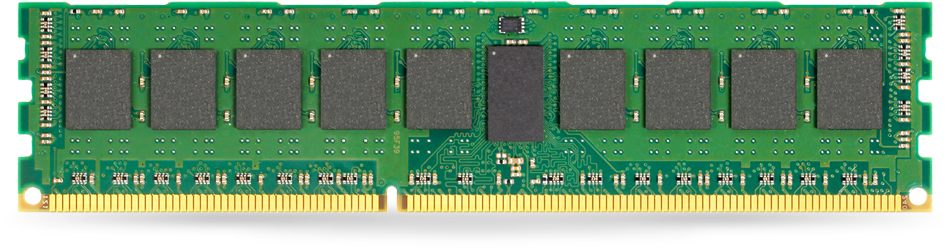
\includegraphics[height = .3\textheight]{DRAM_ddr4}
      };

      \node<2-4>[inner sep = 0] (dram_0) {
        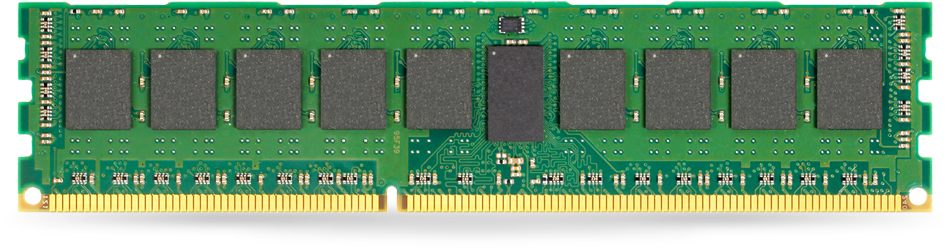
\includegraphics[height = .2\textheight]{DRAM_ddr4}
      };

      \node<2-4>[inner sep = 0, below = of dram_0] (dram_1) {
        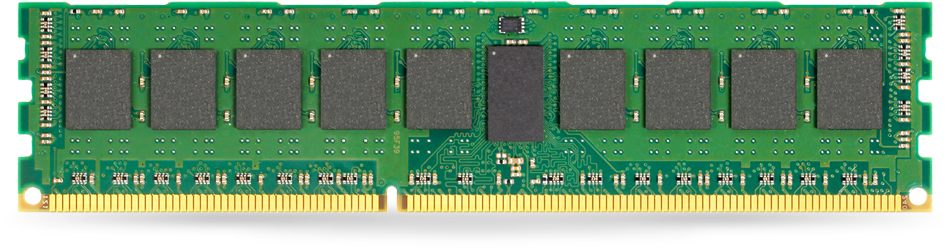
\includegraphics[height = .2\textheight]{DRAM_ddr4}
      };

      \node<2-4>[
      inner sep = 0,
      left = 2cm of $(dram_0.west)!.5!(dram_1.west)$,
      ] (cpu) {
        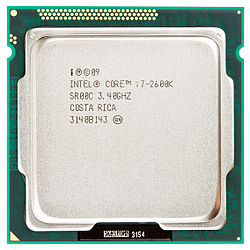
\includegraphics[height = .3\textheight]{cpu}
      };

      \draw<2-4> (cpu) -- ++(2, 0) -- ++(0, 1)  |- node[above] {Channel 0} (dram_0.west);
      \draw<2-4> (cpu) -- ++(2, 0) -- ++(0, -1) |- node[below] {Channel 1} (dram_1.west);

      \node<3-4>[
      right = 0.1 of dram_0,
      ] (rank_0) {
        Front of DIMM:\\rank 0
      };

      \draw<3-4> (dram_0) to [out = 80, in = 60, looseness = 8] node[above] {Back of DIMM: rank 1} (dram_0);
      \draw<3-4> (dram_0) -> (rank_0);

      \draw<4>[red,
      rounded corners,
      very thick,
      ] (2.25, -2.9) rectangle (2.85, -2.1);

      \node<4> (chip_capt) at (3.5, -2.4) {Chip};

      \node<5>[bank,
      ] (bank_0) {
        Row 0
        \nodepart{two}
        Row 1
        \nodepart{three}
        $\cdots$
        \nodepart{four}
        Row 32767
        \nodepart{five}
      };

      \node<5>[
      draw,
      below = .1 of bank_0,
      rectangle,
      fill = Blue,
      text = White,
      ] (r_buf_0) {
        Row buffer
      };

      \node<5>[
      fit = (bank_0) (r_buf_0),
      draw,
      label = above:Bank 0,
      ] {};

      \node<5>[bank,
      right = of bank_0,
      ] (bank_1) {
        Row 0
        \nodepart{two}
        Row 1
        \nodepart{three}
        $\cdots$
        \nodepart{four}
        Row 32767
        \nodepart{five}
      };

      \node<5>[
      draw,
      below = .1 of bank_1,
      rectangle,
      fill = Blue,
      text = White,
      ] (r_buf_1) {
        Row buffer
      };

      \node<5>[
      fit = (bank_1) (r_buf_1),
      draw,
      label = above:Bank 1,
      ] {};


      \node<5>[bank,
      right = of bank_1,
      ] (bank_n) {
        Row 0
        \nodepart{two}
        Row 1
        \nodepart{three}
        $\cdots$
        \nodepart{four}
        Row 32767
        \nodepart{five}
      };

      \node<5>[
      draw,
      below = .1 of bank_n,
      rectangle,
      fill = Blue,
      text = White,
      ] (r_buf_n) {
        Row buffer
      };

      \node<5>[
      fit = (bank_n) (r_buf_n),
      draw,
      label = above:Bank n,
      ] {};

      \node<5>[
      rectangle,
      draw,
      fill = ForestGreen,
      text = White,
      minimum width = 2cm,
      minimum height = 2cm,
      above = of bank_1,
      label = above:Chip,
      ] (chip) {
        Bank 0\\
        Bank 1\\
        $\cdots$\\
        Bank n
      };

      \node<6>[
      rectangle split,
      rectangle split parts = 5,
      rectangle split horizontal,
      text = White,
      fill = ForestGreen,
      draw,
      label = above:Row of DRAM,
      ] (dram_row) {
        Cell 0
        \nodepart{two}
        Cell 1
        \nodepart{three}
        Cell 2
        \nodepart{four}
        $\cdots$
        \nodepart{five}
        Cell n
        \nodepart{six}
      };

      \node<6>[
      below = of dram_row,
      ] (cap) {
        Capacitor
      };

      \draw<6> (cap) -> (dram_row.one south);
      \draw<6> (cap) -> (dram_row.two south);
      \draw<6> (cap) -> (dram_row.three south);
      \draw<6> (cap) -> (dram_row.five south);

    \end{tikzpicture}
    % \caption{DRAM organization}\label{dram_arch}
  \end{figure}

  \note<1>{

    Для повышения производительности работы с DRAM были использованы те же
    методы, что и в случае с кэшем. Современные компьютерные системы
    организовывают DRAM в виде \textbf{каналов}, \textbf{DIMM (Dual Inline
      Memory Modules)}, \textbf{рангов} и \textbf{банков}.

    Количество памяти увеличивается в разы при перемножении количества банков на
    количество \textbf{DIMM модулей}.

  }

  \note<2>{

    Для \textbf{увеличения ширины потока данных} и увеличения количества
    параллельных потоков современные компьютерные системы используют
    \textbf{несколько каналов}. Каждый канал управляется независимо и
    параллельно через DRAM шину.

  }

  \note<3>{

    Современные модели DRAM имеют обычно от \textbf{1 до 4 рангов}, количество
    которых увеличивается при перемножении с количеством банков. Такого рода
    параллелизм позволяет \textbf{уменьшить промах строки}.

  }

  \note<5>{

    Каждый из этих банков имеет своё собственное состояние и может иметь
    \textbf{независимо от других банков} открытую строку.

    Современная DDR3 DRAM память имеет 8 банков, а DDR4 DRAM 16 банков (на
    ранг).

  }

  \note<6> {

    В случае если два адреса \textbf{отображаются на пространство одного и того
      же} DIMM модуля, ранга и банка, то эти адреса физически
    \textbf{расположены рядом друг с другом} в DRAM. В таких случаях два адреса
    оказываются в банке с одним и тем же номером. В случае, если адреса
    отображаются на пространство банков с одним и тем же номером, но разных
    рангов или DIMM'ов, то они не расположены физически рядом.

    Также как и с кэшем, существуют функции, которые производят отображение
    физического адреса на конкретные канал, DIMM, ранг и банк. Как работают эти
    функции, публично известно только у AMD, Intel не публиковала никакой
    информации. Однако, относительно недавно (2015, 2016) был произведён
    реверс-инжиниринг данных функций. Знание того, \textbf{как производится
      отображение физического адреса на физические структуры} даёт нам новый
    вектор атак --- \textbf{атаки по сторонним каналам на DRAM}.

  }

\end{frame}